\begin{figure}[t]
\centering

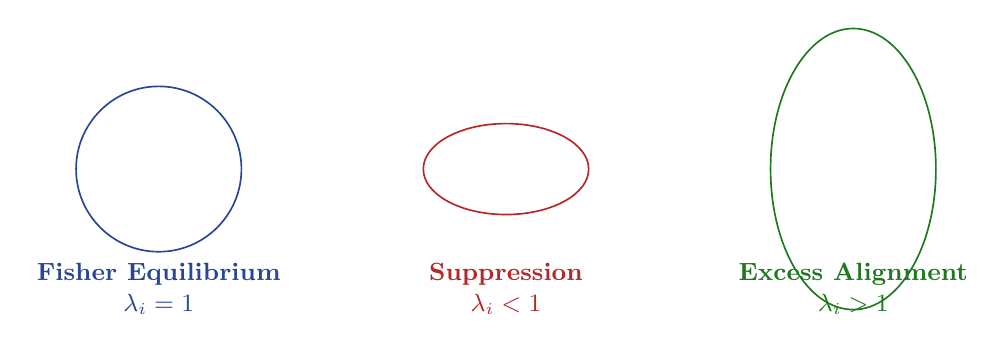
\begin{tikzpicture}[scale=1.05]

    % Colors in a more professional physics palette
    \definecolor{eqcol}{RGB}{40,70,150}
    \definecolor{supcol}{RGB}{180,40,40}
    \definecolor{excol}{RGB}{30,120,30}

    % Common text style
    \tikzset{
        reglabel/.style={font=\small\bfseries, align=center}
    }

    % ============== Fisher equilibrium (circle) ==============
    \begin{scope}[xshift=0cm]
        \draw[semithick, eqcol] (0,0) circle (1cm);
        \node[eqcol, reglabel] at (0,-1.45)
            {Fisher Equilibrium\\$\lambda_i = 1$};
    \end{scope}

    % ================== Suppression ellipse ==================
    \begin{scope}[xshift=4.2cm]
        \draw[semithick, supcol] (0,0) ellipse (1cm and 0.55cm);
        \node[supcol, reglabel] at (0,-1.45)
            {Suppression\\$\lambda_i < 1$};
    \end{scope}

    % ================= Excess Alignment ellipse ==============
    \begin{scope}[xshift=8.4cm]
        \draw[semithick, excol] (0,0) ellipse (1cm and 1.7cm);
        \node[excol, reglabel] at (0,-1.45)
            {Excess Alignment\\$\lambda_i > 1$};
    \end{scope}

\end{tikzpicture}

\caption{
Geometric regimes of empirical alignment on a Fisher manifold.
Equilibrium corresponds to isotropic curvature ($\lambda_i=1$),
suppression reflects contraction of sensitivity along one or more axes
($\lambda_i<1$), and excess alignment corresponds to expansion beyond
the Fisher baseline ($\lambda_i>1$).
}
\label{fig:alignment-regimes}
\end{figure}
